% Editable reconstruction; interpretation recorded in root.json.
% Shared standalone design for the editable figure reconstructions.
\documentclass[tikz,border=5pt,10pt]{standalone}
\usepackage[T1]{fontenc}
\usepackage[utf8]{inputenc}
\usepackage{newpxtext,newpxmath}
\usepackage[scaled=.94]{sourcesanspro}
\usepackage{pgfplots}
\pgfplotsset{compat=1.18}
\usetikzlibrary{arrows.meta,calc,positioning,decorations.pathreplacing,
  decorations.markings,patterns,matrix,shapes.geometric,fit,backgrounds,
  intersections,angles,quotes}
\definecolor{ink}{HTML}{203746}
\definecolor{accent}{HTML}{146C78}
\definecolor{muted}{HTML}{667780}
\definecolor{signalred}{HTML}{B94B44}
\color{ink}
\tikzset{>=Latex,line width=.8pt,
  every node/.style={font=\small},
  axis/.style={->,draw=muted,line width=.5pt},
  guide/.style={draw=muted,dashed,line width=.45pt},
  curve/.style={draw=accent,line width=1pt},
  marker/.style={circle,fill=accent,inner sep=1.5pt},
  labelbox/.style={fill=white,inner sep=2pt}}

\begin{document}

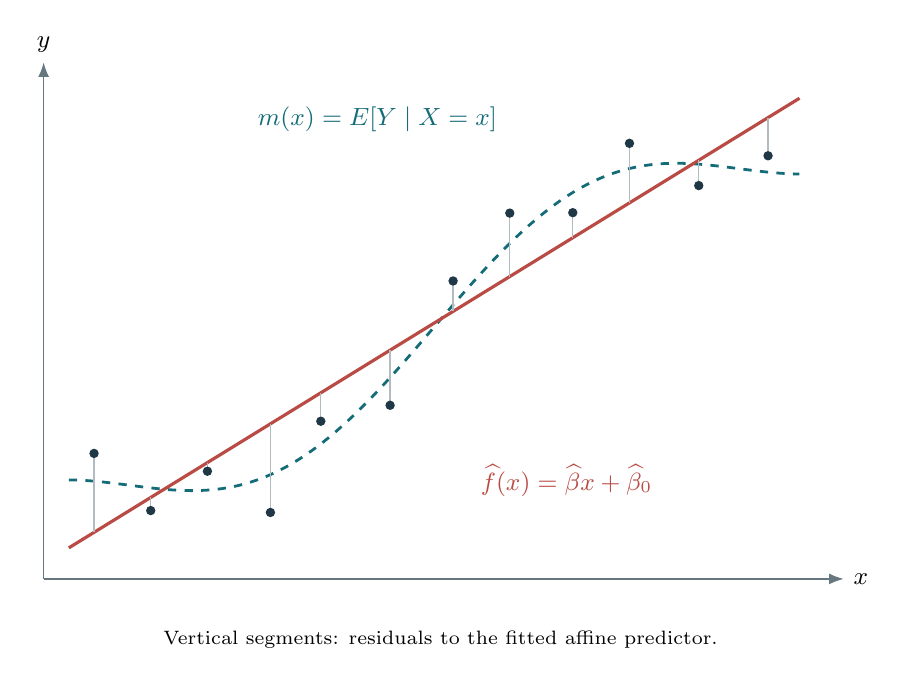
\begin{tikzpicture}[x=1.6cm,y=1.6cm]
\draw[axis] (-3.1,-2)--(3.25,-2) node[right] {$x$};
\draw[axis] (-3.1,-2)--(-3.1,2.1) node[above] {$y$};
\draw[accent,dashed,line width=1pt,domain=-2.9:2.9,samples=140] plot (\x,{.52*\x+.5*sin(deg(1.3*\x))});
\draw[signalred,line width=1.15pt,domain=-2.9:2.9] plot (\x,{0.6153725024*\x+0.0310167444});
\draw[muted!50,line width=.45pt] (-2.7,-1.0039350)--(-2.7,-1.6304890);\fill[ink] (-2.7,-1.0039350) circle(1.7pt);
\draw[muted!50,line width=.45pt] (-2.25,-1.4574516)--(-2.25,-1.3535714);\fill[ink] (-2.25,-1.4574516) circle(1.7pt);
\draw[muted!50,line width=.45pt] (-1.8,-1.1452324)--(-1.8,-1.0766538);\fill[ink] (-1.8,-1.1452324) circle(1.7pt);
\draw[muted!50,line width=.45pt] (-1.3,-1.4724518)--(-1.3,-0.7689675);\fill[ink] (-1.3,-1.4724518) circle(1.7pt);
\draw[muted!50,line width=.45pt] (-0.9,-0.7483753)--(-0.9,-0.5228185);\fill[ink] (-0.9,-0.7483753) circle(1.7pt);
\draw[muted!50,line width=.45pt] (-0.35,-0.6217312)--(-0.35,-0.1843636);\fill[ink] (-0.35,-0.6217312) circle(1.7pt);
\draw[muted!50,line width=.45pt] (0.15,0.3648833)--(0.15,0.1233226);\fill[ink] (0.15,0.3648833) circle(1.7pt);
\draw[muted!50,line width=.45pt] (0.6,0.9036397)--(0.6,0.4002402);\fill[ink] (0.6,0.9036397) circle(1.7pt);
\draw[muted!50,line width=.45pt] (1.1,0.9070523)--(1.1,0.7079265);\fill[ink] (1.1,0.9070523) circle(1.7pt);
\draw[muted!50,line width=.45pt] (1.55,1.4574766)--(1.55,0.9848441);\fill[ink] (1.55,1.4574766) circle(1.7pt);
\draw[muted!50,line width=.45pt] (2.1,1.1220347)--(2.1,1.3232990);\fill[ink] (2.1,1.1220347) circle(1.7pt);
\draw[muted!50,line width=.45pt] (2.65,1.3586132)--(2.65,1.6617539);\fill[ink] (2.65,1.3586132) circle(1.7pt);

\node[accent,fill=white] at (-.45,1.65) {$m(x)=\mathbb E[Y\mid X=x]$};
\node[signalred,fill=white] at (1.05,-1.22) {$\widehat f(x)=\widehat\beta x+\widehat\beta_0$};
\node[font=\scriptsize] at (.05,-2.48) {Vertical segments: residuals to the fitted affine predictor.};
\end{tikzpicture}
\end{document}
